%%%%%%%%%%%%%%%%%%%%%%%%%%%%%%%%%%%%%%%%%%%%%%%%%%%%%%%%%%%%%%%%%
\section{Altitude Effects}
%%%%%%%%%%%%%%%%%%%%%%%%%%%%%%%%%%%%%%%%%%%%%%%%%%%%%%%%%%%%%%%%%

The thermodynamic state of the atmosphere changes with altitude, thereby affecting the aircraft performance (thrust and lift, etc). 

The temperature in the atmosphere follows a complicated function (see \cref{FIG_ALTITUDE}), in which different physical processes become important (such as buoyancy and radiation, etc) in controlling the ambient state at different altitude. 

%================================================================
\begin{figure}[!h!]
  \begin{center}
    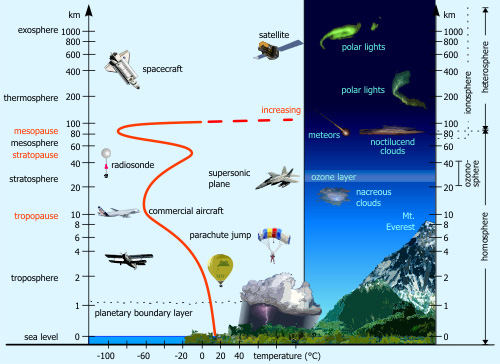
\includegraphics[width = 0.95\textwidth]{atmosphere}
  \end{center}
  \caption{\label{FIG_ALTITUDE}Earth atmosphere (source: \url{www.theozonehole.com}).}
\end{figure}
%================================================================

Since the flight altitude of airbreathing vehicles is limited by constraints on the required lift (density), available oxygen concentration, and environmental impact and emissions, we restrict our analysis to the troposphere ($h\le 12$ km). To good accuracy, this layer can be characterized by an isotropic process, and from a force balance between buoyancy and pressure forces acting on a differential control volume, we can derive the following altitude-dependent state relation for temperature $T(z)$, density $\rho(z)$, and pressure $p(z)$:
\begin{subeqnarray}
  \f{T(z)}{T_s} &=& \left[1-\f{\gamma-1}{\gamma}\left(\f{z}{\wt{z}}\right)\right]\\
  \f{\rho(z)}{\rho_s} &=& \left[1-\f{\gamma-1}{\gamma}
                          \left(\f{z}{\wt{z}}\right)\right]^{\f{1}{\gamma-1}}\\
  \f{p(z)}{p_s} &=& \left[1-\f{\gamma-1}{\gamma}\left(\f{z}{\wt{z}}\right)\right]^{\f{\gamma}{\gamma-1}}
\end{subeqnarray}
where
\begin{equation}
  \wt{z} = \f{p_s}{\rho_s g}\, \text{,}
\end{equation}
and $p_s=101$,325 Pa, $\rho_s=1.23$ kg/m$^3$, and $T_s=288$ K.

A comparison of the isentropic model with the International Standard Atmosphere (ISA) is shown in Fig.~\ref{FIG_ISAISENCOMPARE}. The ISA model is created by presuming a temperature profile (piece-wise linear for the altitudes shown), and computing the pressure and density from the hydrostatic pressure distribution and ideal gas law. That is,

\begin{equation}
	\begin{aligned}
		\frac{\d p}{\d z}&=-\rho g\ , \\
		\rho &= \frac{p}{RT(z)}.
	\end{aligned}
\end{equation}
Combining and integrating, one obtains
\begin{equation}
	\begin{aligned}
		\frac{p(\hat z)}{p_\mathrm{s}}=\exp\left(-\int_0^{\hat z} \frac{T_\mathrm{s}}{T(\hat z')}\d \hat z'\right)\ ,
	\end{aligned}
\end{equation}
where $\hat z=z/\tilde z$ is used for brevity.

As shown in the figure, the two models follow rather closely for the density and pressure but not the temperature. MATLAB contains the function "atmosisa", which gives the ISA model's thermodynamic conditions as a function of altitude. It is recommended that this function be used in the homework .

%================================================================
\begin{figure}[!h!]
	\begin{center}
		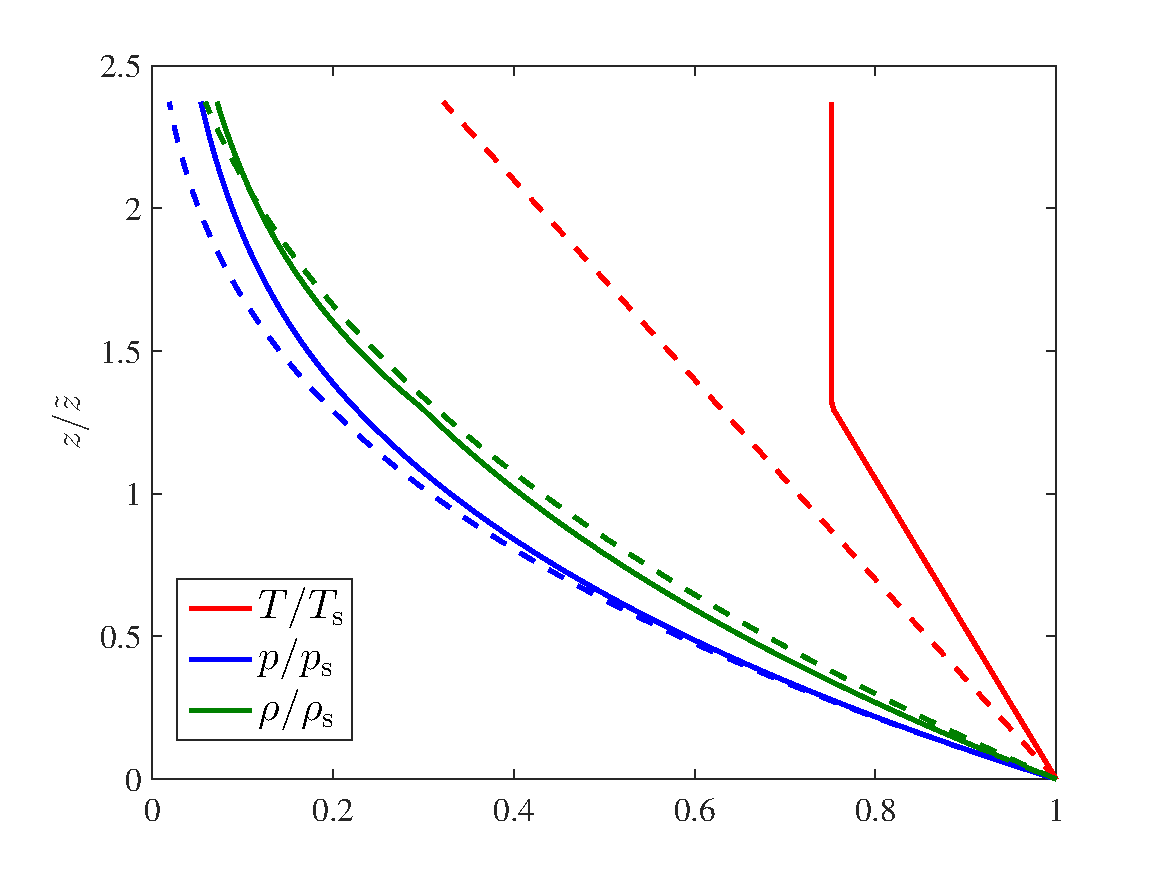
\includegraphics[width = 0.95\textwidth]{atmosphericPropertiesComparison.pdf}
	\end{center}
	\caption{\label{FIG_ISAISENCOMPARE} The ISA model (--) compared against the isentropic model (- -).}
\end{figure}
%================================================================